\chapter{Implementation}
% IFØLGE JIM ER DET HER FISKEN HENTES TILBAKE PÅ LAND (BLANT ANDRE STEDER).
% SE PÅ TØNNES SIN MASTEROPPGAVE OG 'Archive History' NEDERST I DOKUMENTET FOR INSPIRASJON.






\section{The musical multi-robot system}
% First intro-explanation (where the oscillator talk is introduced):
Envision that we have a multi-agent collective scenario consisting of musical robots, modelled as oscillators, entraining to synchronize to each other solely based on audio signals they themselves transmit when being at their oscillator-peak (i.e. having phase $\phi(t)=1$). All agents have the ability to listen for such transmitted \textit{fire-signals} from their neighbours, which they then will use as a trigger to adjust themselves according to some well-designed update-functions. The goal and target state of the system is \textit{harmonic synchrony}, as K. Nymoen et al. \cite{nymoen_synch} coined it when ...

% First figure to get a quick idea of what the system does:
% MÅ FIKSE ELLER FJERNE!!!!!:
	% - Fjern den Gule/Orange Dr. Squiggle'n fra Spawne-lista (pga. tvetydighet pga. gul fire-color).
	% - Få god oppløsning og kanskje bruke .PNG istedenfor .JPG.
	% - Ikke skape misoppfatningen om at alle agenter må fyre samtidig for å være *harmonisk* synkroniserte.
		% + SKAL JEG KANSKJE BARE DROPPE HELE DENNE FIGUREN SIDEN DEN PÅ EN MÅTE BARE GJØR DETTE?
\begin{figure}[h]
	\centering
		\begin{subfigure}[t]{.5\textwidth}
			\centering\captionsetup{width=.9\linewidth}%
			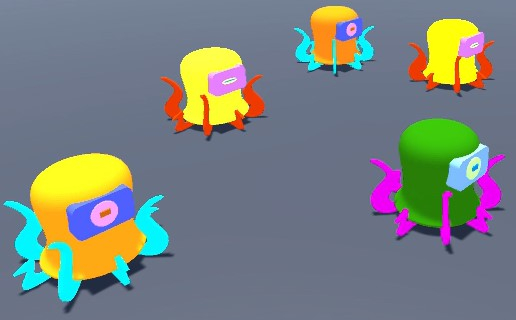
\includegraphics[width=0.9\linewidth]{Assets/Figures/IntroUnsynch.jpg}
			\caption{The agents firing asynchronously at first. Here, only the two Dr. Squiggles with red tentacles are firing simultaneously, but the rest are not.}
			\label{initial:unsynch}
		\end{subfigure}%
		\begin{subfigure}[t]{.5\textwidth}
			\centering\captionsetup{width=.9\linewidth}%
			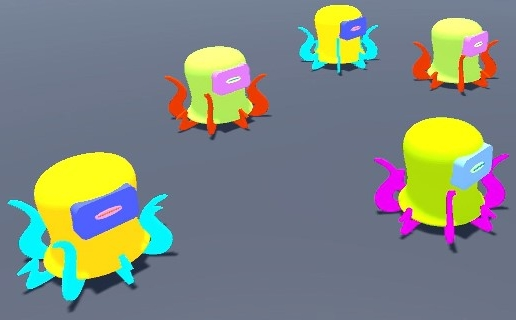
\includegraphics[width=0.9\linewidth]{Assets/Figures/IntroSynch.jpg}
			\caption{Seconds later, after having listened to each other's fire-event signals and adapted themselves accordingly, the agents are here firing synchronously.}
			\label{initial:synch}
		\end{subfigure}
	\caption{Synchronization (of phases) in a musical robot collective achieved.}	% Gammel caption: "The musical agents, also known as M. J. Krzyzaniak's Dr. Squiggles, are actively listening for signals from each other's fire-events, entraining to synchronize to each other accordingly." Cite Pierre her?
	\label{initial:synch}
\end{figure}





% Considerations:
\besk{"Det man har utviklet" — Kyrre}

\gjor{
	\textbf{Svar på disse spørsmålene (kompilert fra Tønnes sin masteroppgave):}
	What does the chapter do? What's the main goal of the design/implementation/developed system? What do these goals require? Why did you make the design-choices you made? What advantages do these choices ensure/enable? Give a short chapter-outline (perhaps first about the design, my additional Self-Awareness component, manual choice of initial parameters, and then the benchmark or målestokk or performance measure I use to evaluate with).
}

\gjor{Skriv opp Worklog-materiale dandert i henhold til gode master-theses}

% Archive History:

	% \section{Benchmark}
		% \besk{Her jeg beskriver Nymoens algoritmer og formler (originalt), men \opphoy{sånn jeg har implementert det i Unity}}
	
		% \gjor{Vurder om 'Benchmark' bør deles opp i sin egen sub-seksjon i det hele tatt — eller f.eks. slås sammen med 'Proposed Algorithm'}
	
		% \besk{(Hentet fra Samuelsens master?) Presentering av metoden brukt til å evaluere ytelsen av den foreslåtte/proposed'e algoritmen. Først er kanskje en referanse-algoritme brukt for sammenlikning beskrevet. Deretter er (f.eks. objektiv-) funksjoner brukt i testene forklart. Endelig (til slutt) er kanskje miljøene/environments'a og parameterne brukt presentert}
		
		
	% \section{Proposed Algorithm}
		% \besk{Evt. her jeg skriver om Self-Awareness-komponenten(e) jeg legger til ang. Belief-awareness og/eller Expectation-awareness (jf. det jeg og Kyrre snakka om Mid-November på 'reMarkable -> Møter -> ROBIN -> Kyrre')}
	
		% \gjor{Vurder om 'Proposed Algorithm' bør deles opp i sin egen sub-seksjon i det hele tatt — eller f.eks. slås sammen med 'Benchmark'}
	